\section{What cannot be detected: impossibility and the visibility boundary}
\label{sec:blindness}

Section~\ref{sec:detection} mapped what the calibrated alarm sees and at what strength. This section maps the complement: which statistic classes cannot see sub-threshold dense confounding, where the exact boundary sits, and where our own universal claims broke under pre-registered falsification and had to be rescoped. The bookkeeping matters as much as the theorems, so the class map comes first.

\subsection{Statistic classes, and what impossibility can mean}

\begin{remark}[Trivial layer]
\label{rem:purex}
Statistics depending on $(Y,X)$ only through $\mathrm{spec}(X_c^\top X_c/n)$ are independent of $\gamma$ under every model in play, so power equals size identically. Scree alarms live here. Their blindness to confounding is a data-processing identity, not an asymptotic statement, and we record it as a remark so that it cannot masquerade as a finding.
\end{remark}

The substantive class comprises augmented-spectrum alarms: statistics measurable with respect to the spectrum of the sample second-moment matrix of the standardized pair,
\[
M_{\mathrm{aug}}=\begin{pmatrix}1 & \hat w^\top\\ \hat w & \hat\Sigma\end{pmatrix},
\]
that is, eigenvalue functionals of the whitened cross-moment structure. What can be proved about this class at population level is the following boundary.

One normalization is used throughout the statement: the $\Sigma_X\beta$ component of the augmented first coordinate contributes only $O_p(p^{-1/2})$ to each coupling under A4a and is therefore omitted from $\kappa_j$; its bulk-spread remainder perturbs the absolutely continuous part alone, which part (iii) covers.

\begin{proposition}[Population detachment boundary]
\label{prop:detach}
Fix a subcritical profile ($l_j<\sqrt c$ for all $j$), fixed $r$, and Haar loadings, with response standardization in force, and let $\sigma_y^2(g)=A+g^2$. The population secular equation for a detached level $\tau\notin\mathrm{spec}(\Omega)$ of the standardized pair is
\[
\tau=1+\sum_{j\le r}\frac{\kappa_j}{\tau-\tau_j},
\qquad
\kappa_j=\frac{l_j\,g_j^2}{\sigma_y^2(g)},\quad g_j=g\,\mathrm{dir}_j,
\]
with population spikes $\tau_j=1+l_j$ and bulk edges $b_\pm=(1\mp\sqrt c)^2$. Then: (i) on the top edge, $\tau-1-\sum_j\kappa_j/(\tau-\tau_j)$ is strictly increasing on $(b_+,\infty)$, so a detached level exists iff
$\omega_e:=\sum_j l_j\,\mathrm{dir}_j^2/(c+2\sqrt c-l_j) > B:=c+2\sqrt c$,
so at strength $g$ a detached level exists iff $\{g^2/(A+g^2)\}\,\omega_e>B$; since $g^2/(A+g^2)$ increases toward $1$, detachment is possible at some strength iff $\omega_e>B$, and it then persists for all sufficiently large $g$. For the scaling sub-profiles used throughout this paper the ratio satisfies $\omega_e/B = 0.235$, $0.081$, and $0.036$ at $c=0.2$, $0.8$, and $2.0$, so no detached level ever exists at any strength; (ii) below the bulk exactly one root exists for every nonzero coupling, sticking to $b_-$ as the coupling vanishes. The root can separate by unit depth only if the coupling pull at the edge exceeds the depth scale, the wake criterion $(1-b_-)\bigl((1+\bar l)-b_-\bigr)<\omega$ for equal spikes $\bar l$ with saturated couplings (evaluated as $g\to\infty$, where $g^2/(A+g^2)\to1$); this necessary condition fails at every studied equal-spike scaling cell, the attained left side exceeding the allowed right side by $0.64$ versus $0.22$, $1.42$ versus $0.45$, and $1.27$ versus $0.71$ across the three subcritical aspect ratios; (iii) inside the no-detachment region the limiting empirical spectral distributions under null and alternative coincide, by finite-rank invariance of the absolutely continuous part.
\end{proposition}

\begin{proof}[Proof sketch]
Each claim is elementary. For (i), strict monotonicity follows from $\sum_j\kappa_j/(\tau-\tau_j)^2>0$ on $(b_+,\infty)$ where all denominators are positive, and evaluating the secular inequality as $\tau\downarrow b_+$ collapses the existence condition to the displayed ratio with the coupling scale cancelling through $\sigma_y^2(g)$; part (ii) is the mirror computation at the lower edge with its wake inequality $(1-b_-)((1+l)-b_-)<\omega$ for equal spikes; part (iii) is finite-rank perturbation invariance of the absolutely continuous spectrum. Full details are archived in the released theory notes.
\end{proof}

The proved boundary concerns population roots. A stronger claim suggests itself: that below it, the entire laws of $\mathrm{spec}(M_{\mathrm{aug}})$ are mutually contiguous in the sense of Onatski--Moreira--Hallin \citep{onatski2013asymptotic}, which via Le Cam's two-point lemma would imply that no test measurable with respect to $\mathrm{spec}(M_{\mathrm{aug}})$ has asymptotic power exceeding size. Below the BBP threshold the overlap between sample spikes and the coherent confounding direction collapses at rate $n^{-1/2}$ \citep{benaychgeorges2012singular}, and under response standardization the effective first-coordinate spike carries $\sigma_y(g)^{-1}$ in its denominator, so self-normalization pushes detectability down precisely as the confounder grows; the OMH contiguity machine, developed for sphericity-plus-rank-one alternatives, looks tailor-made. We announce this planned claim only to audit it: as reported next, its pre-registered falsifier destroyed it, and the subsection closes with the layered statement that actually survives.

What is claimed, and what is not, must be fenced explicitly. First, every impossibility statement here is statistic-class-scoped and never information-theoretic: contiguity arguments themselves produce a strictly positive likelihood-ratio power envelope near the threshold, so information-theoretic detectability below the BBP boundary remains possible in principle, and our certificates bind named classes only. Second, pure-X blindness is the trivial Remark~\ref{rem:purex}. Third, and most important for honest reporting: the strong version of the augmented-class claim, mutual contiguity of the full spectrum $\mathrm{spec}(M_{\mathrm{aug}})$ throughout the no-detachment region, was fed to our own pre-registered falsifiers and did not survive.

The falsifiers are worth reading. Fresh-draw Mann-Whitney AUCs of the true $\lambda_{\max}(M_{\mathrm{aug}})$ at $(c=0.2$, subcritical profile, $\theta=\pi/6)$ fall consistently toward perfection, from $0.286$ to $0.051$ at $g=3.2$ and from $0.351$ to $0.133$ at $g=1.6$ as $n$ runs from $800$ to $3200$: separation is consistent and downward, the opposite of contiguity. At the visibility fixed point derived below ($\theta=\pi/2$, equal subcritical spikes, so $\omega=\omega_\star$), the cross-moment mass is flat ($0.7014$ versus $0.7066$) and every bulk spectral functional is flat, yet the augmented root separates upward with AUC $0.998$ and $1.000$ at $n=1600$ and $3200$, $g=3.2$. Neither observation contradicts Proposition~\ref{prop:detach}: no population root detaches from the bulk in either configuration, and the limiting bulk distributions coincide, exactly as part (iii) says; what separates is the finite-sample top coordinate, carried by fluctuations that self-normalization through $\sigma_y(g)$ makes geometry-dependent rather than mass-dependent, a signature with no analogue in the OMH alternative. Contiguity therefore fails precisely where the population picture looks most blind, which is why the planned universal claim died while the boundary theorem survived intact. A pipeline erratum compounds the history: the frozen S1 implementation silently inverted its secular bracket whenever the bracketing discriminant turned negative, which is common at $c\le 1$, returning a degenerate surrogate correlated with $\lambda_{\max}(\hat\Sigma)$. Every stored S1 artifact therefore reads ``surrogate-S1'', and gate verdicts are unaffected because S1 was demoted to diagnostic before any sweep data existed, with self-consistent Monte Carlo thresholds.

The impossibility statement that ships is layered. It is airtight for pure-X alarms by identity; it holds, proved via Proposition~\ref{prop:ceiling} and confirmed in $9$ of $9$ blind strata, for the spike-coordinate calibrated class S2; and it is false as a universal claim for $\mathrm{spec}(M_{\mathrm{aug}})$, which in fact detects subcritical confounding with a geometry-dependent direction. Every decoupling claim in this paper cites these scopes. The alignment stress test sharpens the geometric point (Figure~\ref{fig:alignment}): sweeping $\theta$ at fixed profile and strength over twelve configurations of $800$ replicates each, S2 power holds at $1.000$ at every angle except exactly $\theta=\pi/2$, where it collapses to $0.022$, while the principal-component $F$ baseline falls only to $0.262$. Detection tracks supercritical-aligned mass, never total confounding.

\begin{figure}[t]
\centering
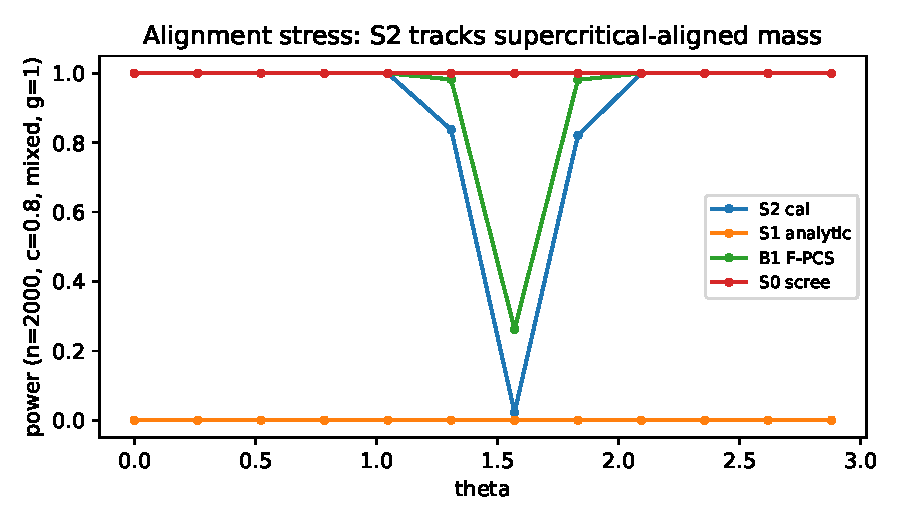
\includegraphics[width=0.85\textwidth]{figures/alignment_stress.pdf}
\caption{Alignment stress test: detection power against the alignment angle $\theta$ of the confounding direction, from $\theta=0$ (strongest factor) to $\theta=\pi/2$ (weakest reported factor). The calibrated alarm S2 collapses only at exact subcritical alignment ($\theta=\pi/2$: power $0.022$), while the principal-component $F$ baseline retains $0.262$. Size is $\theta$-invariant by construction.}
\label{fig:alignment}
\end{figure}

\subsection{An exact visibility boundary for quadratic probes}

Eigenvalue alarms aside, the cheapest summary of $(\tilde Y,X_c)$ is quadratic. This subsection analyzes the single carrier defined next; broader concentrated quadratic functionals follow the same algebra. One sign convention is fixed now: carrier AUCs are quoted on the deflation side established below, so an AUC below $1/2$ indicates separation with negative orientation, and we flag where the flipped reading matters. Take as carrier $q(\tilde Y,X_c)=\|\hat w\|^2$, with $\hat w=X_c^\top\tilde Y/n$ the fully self-standardized cross-moment, $\tilde Y=Y_c/\mathrm{sd}_y$, and write $q_{\mathrm{raw}}=\|X_c^\top Y_c/n\|^2$ for its pre-standardization counterpart. Write $\omega=\sum_j l_j\,\mathrm{dir}_j^2=\|\Lambda\,\mathrm{dir}\|^2$ for the per-unit-strength confounding mass and $A=1+\sigma_\varepsilon^2$.

\begin{proposition}[Visibility law]
\label{prop:visibility}
As $n,p\to\infty$ with $c=p/n$ fixed under Haar loadings,
\[
v_0:=\lim\mathbb{E}\,\mathrm{sd}_y^2\big|_{H_0}=A,
\qquad
M_0:=\lim\mathbb{E}\big[q_{\mathrm{raw}}\,\big|\,H_0\big]=1+cA,
\]
where $q_{\mathrm{raw}}$ is as defined above the proposition. Moreover, at link strength $g$ along direction $\mathrm{dir}$,
\[
\mathbb{E}[q\mid g]\;\longrightarrow\;\frac{M_0+g^2(\omega+c)}{v_0+g^2}
\;=\;m_0-\frac{g^2(\omega_\star-\omega)}{v_0+g^2},
\qquad
m_0=\frac{M_0}{v_0},\qquad
\omega_\star=\frac{1}{A}.
\]
Finally, fix a detection target $\mathrm{AUC}^{\star}\in(1/2,1)$ and let $a(\mathrm{AUC}^{\star}):=\sqrt2\,\Phi^{-1}(\mathrm{AUC}^{\star})\,\mathrm{sd}_0(q_0)$ be the standardized separation it requires under the single-carrier Gaussian envelope, where $\mathrm{sd}_0(q_0)$ is the null standard deviation of the carrier. The carrier probe $(q,\mathrm{sd}_y)$ is born blind iff
$|\omega-\omega_\star|\le a(\mathrm{AUC}^{\star})$;
otherwise the visibility threshold solves $g_{\mathrm{vis}}^2=a(\mathrm{AUC}^{\star})\,v_0/\{\upsilon-a(\mathrm{AUC}^{\star})\}$ with headroom $\upsilon=\omega_\star-\omega>0$.
\end{proposition}

The raw floor in the first display follows from a trace identity for the Haar-$\beta$ piece plus $\sigma_\varepsilon^2 c$ for the noise piece; under $H_1$ the numerator gains $g^2(\omega+c)$ (coherent mass plus bulk leakage) while division by the realized response scale contributes the denominator. The derivation of all displayed laws is given in Appendix~\ref{app:sec5proofs}. The standardized shift $\Delta(g)=\mathbb{E}[q\mid g]-m_0$ therefore satiates: $\sup_g|\Delta(g)|=|\omega_\star-\omega|$, approached from whichever side of the fixed point the profile sits.

Every deterministic constant closes within $2\%$ at $n=2000$: measured $v_0$ is $1.9948$ and $2.0114$ against $A=2$ at $c=0.2$ and $0.8$; measured $M_0$ is $1.3986$ and $2.6168$ against $1.4$ and $2.6$; measured $m_0$ is $0.7005$ and $1.3006$ against $0.70$ and $1.30$. The headline is the interaction with the aspect ratio. For the scaling profiles deployed throughout the study, $l_j\propto\sqrt c$, so $\omega=w_0\sqrt c$ with $w_0=0.5$ for the fully subcritical profile and $w_0=2.375$ for the mixed profile at $\theta=\pi/6$. The subcritical profile meets the fixed point exactly at $c=1$: its headroom is $\upsilon_{\mathrm{sub}}(c)=\omega_\star-\omega(c)=w_0(1-\sqrt c)=0.5\,(1-\sqrt c)$, which vanishes there. We state plainly what this coincidence is: with $\omega_\star=w_0$, the general crossing rule places the born-blind aspect ratio at $c_\star=(\omega_\star/w_0)^2$, and our calibration choice $w_0=\omega_\star=1/A$ puts that crossing exactly at the Marchenko-Pastur boundary. The placement is thus a property of the scaling family and its calibration rather than a universal constant, but within this family it is exact, it is where every simulation and benchmark grid lives, and the mechanism (satiation against a fixed null floor) survives any calibration. Beyond the crossing the sign flips, $\omega>\omega_\star$, and $\|\hat w\|^2$ inflates instead of deflating. The mixed profile crosses already at $c=0.044$ and stays visibly signed across the whole tested grid. Measured anchors agree with the class map: $\mathrm{sd}_0(q_0)=0.0331$ and $0.0422$, headrooms $\upsilon=0.276$ and $0.053$, ceiling ratios $|\Delta|_{\max}/\mathrm{sd}_0$ of $8.3$ in the visible class, where AUC tending to $1$ is reached, versus $1.26$ in the blind class, where the single-carrier AUC stalls between $0.18$ and $0.25$ even at $g=3.2$. The stall figures use the deflation-side orientation demanded by the sign map; read with the sign flipped, the same carrier reaches roughly $0.75$--$0.82$ at satiation, so the carrier is not information-free in the blind class, it is sign-misaligned, and the operational-invisibility claim rests on the boosted-tree probe, which exploits shape and still stalls. With Mann-Whitney $\mathrm{AUC}=\Phi(-|\Delta|/(\sqrt 2\,\mathrm{sd}_0))$ on the deflation side, a budget of $a\approx 2.5$ buys $\mathrm{AUC}\approx 0.96$.

\subsection{The Le Cam probe, reported honestly}

The frozen declaration operationalized computational invisibility as AUC $\le 0.55$ for both flexible probes below the claimed frontier, evaluated with gradient-boosted trees on a frozen $14$-feature spectral map (Figure~\ref{fig:lecam}). As a universal statement it failed, and the failure is the most instructive measurement in the study because it splits by aspect. At $c=0.8$ the probe sits at or near chance, AUC between $0.50$ and $0.58$ through $g=0.8$: the upper end marginally exceeds the declared $0.55$ band and should be read as the edge of the plateau rather than inside it. Informativeness arrives only around $g\ge 1.6$ (AUC $0.62$ to $0.78$), so operational invisibility holds at practically relevant strengths, with the plateau boundary quoted honestly. At $c=0.2$ the probe reads the confounding easily, with AUC $0.84$ already at $g=0.15$ and reaching $1.0$. Feature forensics identify the exploited carrier: the only informative feature is $\|\hat w\|^2$, whose mean shift at $(c=0.2,g=0.8)$ is about $-2.2$ standard deviations and negative, because $\sigma_y^2$ inflates faster than the cross-moment mean, exactly the deflation mechanism of Proposition~\ref{prop:visibility}.

Claims were rescoped rather than defended. Subcritical dense confounding is invisible to the eigenvalue-alarm classes everywhere measured, subject to the layering above; it is operationally invisible to concentrated cross-moment functionals in an intermediate-to-high-$c$ regime at $n=2000$, where invisibility means the declared AUC band is met up to its boundary once orientation conventions are fixed (a sign-flipped reading of a blind-class carrier can reach $0.75$--$0.82$, which is why every such claim names both class and convention); and it is not invisible at low $c$. The theory question accordingly upgrades from whether some second-moment statistic can remain blind to characterizing the detectability phase diagram of general second-moment functionals in $(c,g)$, a question the visibility boundary begins to answer for the quadratic carrier.

Two disclosures complete the record. First, the MMD probe was deferred: its median-heuristic bandwidth returned degenerate values on standardized features, an implementation gap recorded as such, leaving the boosted trees as the evaluated probe. Second, at small $g$ the classifier outperforms the mean-shift envelope: at $c=0.2$, $g=0.15$, the measured AUC of $0.845$ exceeds the Gaussian-envelope prediction near $0.53$ because the learner also exploits distributional shape beyond the first moment. The closed-form curve is therefore the lower envelope and the class-map backbone, and per-point small-$g$ AUC prediction is explicitly out of scope. Compared with confounding-strength diagnostics \citep{janzing2018detecting,rendsburg2024consistent}, which estimate magnitude without shipping exact null laws, the contribution here is a calibrated boundary: a stated functional, a stated ceiling, and a stated aspect at which seeing stops.

\begin{figure}[t]
\centering
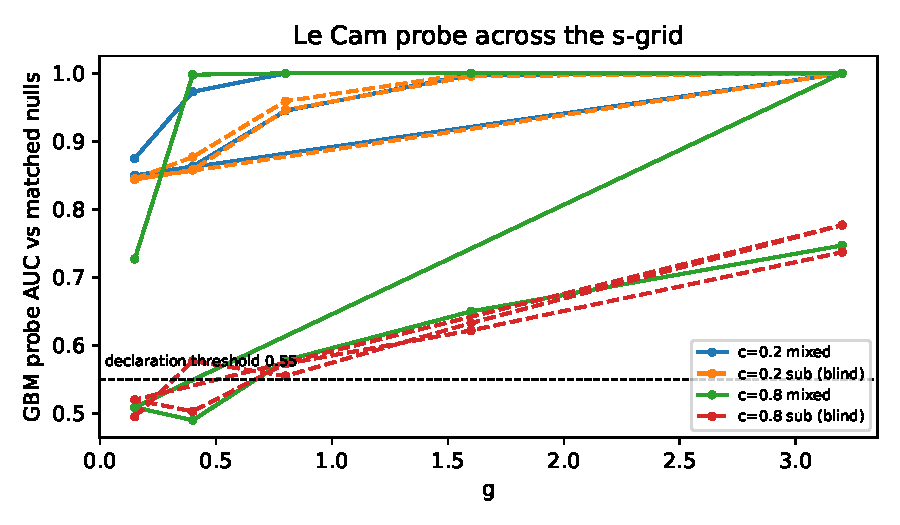
\includegraphics[width=\textwidth]{figures/lecam_probe_auc.pdf}
\caption{Le Cam probe honesty: gradient-boosted AUC against confounding strength $g$ at matched configurations, split by aspect ratio. At $c=0.8$ the probe remains at chance through $g=0.8$ and turns informative only near $g=1.6$; at $c=0.2$ the self-standardized $\|\hat w\|^2$ signature is readable immediately (AUC up to $1.0$). The frozen universal-invisibility rule fails as a universal statement and is rescoped by $c$.}
\label{fig:lecam}
\end{figure}
